\documentclass{article}   	% use "amsart" instead of "article" for AMSLaTeX format

%Predefined definitions
\usepackage{common}

\title{Notes Towards PhD}
\author{Kyle B. Thompson}
%\date{}							% Activate to display a given date or no date

\begin{document}
\maketitle
\section{Adjoint Derivation}

The FUN3D adjoint derivation is given in Eric Nielson's PhD Thesis.  Starting
with forming the Lagrangian as
%------------------------------------------------------------------------------%
\begin{equation}
  L(\md,\mq,\mx,\mathbf{\Lambda})=f(\md,\mq,\mx)
  +\mathbf{\Lambda}^T\mr(\md,\mq,\mx)
\end{equation}
%------------------------------------------------------------------------------%
Where $\mr$ is the residual of the flow equations.  Differentiating with respect
to the design variables $\md$ yields
%------------------------------------------------------------------------------%
\begin{equation}
  \frac{\partial L}{\partial \md}=
  \Bigg\{\frac{\partial f}{\partial \md}+\bigg[\frac{\partial \mx}{\partial \md}\bigg]^T \frac{\partial f}{\partial \mx}\Bigg\}
  +\bigg[\frac{\partial \mq}{\partial \md}\bigg]^T
  \Bigg\{\frac{\partial f}{\partial \mq}+\bigg[\frac{\partial \mr}{\partial \mq}\bigg]^T \mathbf{\Lambda}\Bigg\}
  +\Bigg\{\bigg[\frac{\partial \mr}{\partial \md}\bigg]^T
  +\bigg[\frac{\partial \mx}{\partial \md}\bigg]^T\bigg[\frac{\partial \mr}{\partial \mx}\bigg]^T\Bigg\}\mathbf{\Lambda}
  \label{dL}
\end{equation}
%------------------------------------------------------------------------------%
To eliminate the dependence of conserved variables $\mq$ on the design
variables, we solve the adjoint equation
%------------------------------------------------------------------------------%
\begin{equation}
  \bigg[\frac{\partial \mr}{\partial \mq}\bigg]^T\mathbf{\Lambda}=
  -\frac{\partial f}{\partial \mq}
  \label{adjoint-main}
\end{equation}
%------------------------------------------------------------------------------%
Where the Lagrange multipliers (also known as costate variables),
$\mathbf{\Lambda}$ are the cost function dependence on the residual
%------------------------------------------------------------------------------%
\begin{equation}
  \mathbf{\Lambda}=-\frac{\partial f}{\partial \mr}
\end{equation}
%------------------------------------------------------------------------------%
This can ultimately be used to error estimation and sensitivity analysis for
design optimization.  With the second term in eq.~(\ref{dL}) eliminated, the
derivative of the Lagrangian becomes
%------------------------------------------------------------------------------%
\begin{equation}
  \frac{\partial L}{\partial \md}=
  \Bigg\{\frac{\partial f}{\partial \md}+\bigg[\frac{\partial \mx}{\partial
  \md}\bigg]^T \frac{\partial f}{\partial \mx}\Bigg\}
  +\Bigg\{\bigg[\frac{\partial \mr}{\partial \md}\bigg]^T
  +\bigg[\frac{\partial \mx}{\partial \md}\bigg]^T\bigg[\frac{\partial
  \mr}{\partial \mx}\bigg]^T\Bigg\}\mathbf{\Lambda}
  \label{obj_function}
\end{equation}
%------------------------------------------------------------------------------%
By solving the adjoint equation in \eref{adjoint-main}) to obtain the costate
variable vector, $\mathbf{\Lambda}$, we can now use a non-linear optimizer to
determine the optimum set of design variables, $\md^*$. This can be done using
{\bf PORT} or {\bf KSOPT} in FUN3D, as well as a host of other non-linear
optimizers.

\section{Decoupled Adjoint}

The purpose of this is to show the relationship between the costate variable for total density $\lambda_\rho$ to the costate variables for species densities $\lambda_{\rho_s}$. Beginning with the definition of the Adjoint Equations:
%------------------------------------------------------------------------------%
\begin{equation}
  \left(\frac{\partial R}{\partial Q}\right)^T\lambda = \frac{\partial F}{\partial Q}
  \label{adj_eqn}
\end{equation}
%------------------------------------------------------------------------------%
Where the $R$ is the residual of the governing equations, $Q$ is the vector of conserved variables, and $F$ is the cost function (i.e. lift, drag, etc.). Note that the first term is simply the transpose of the jacobian multiplied by the costate variable vector $\lambda$, and can be written as:
%------------------------------------------------------------------------------%
\begin{equation}
  \left(\frac{\partial R}{\partial Q}\right)_i^T \lambda 
  = \sum_{j=1}^{N_{eq}}{
    \left(\frac{\partial R_j}{\partial Q_i}\right) \lambda_j}
  \label{lhs_sum}
\end{equation}
%------------------------------------------------------------------------------%
Suppose we define the system of equations in two different ways.  The first system, which we'll call the ``meanflow system'', consists of 5 equations:
%------------------------------------------------------------------------------%
\begin{equation}
  R = \begin{pmatrix} 
        R_{\rho} \\ R_{\rho u} \\ R_{\rho v} \\ R_{\rho w} \\ R_{\rho E}
      \end{pmatrix}, \quad
      \lambda = \begin{pmatrix}
        \lambda_\rho \\ \lambda_{\rho u} \\ \lambda_{\rho v} \\ \lambda_{\rho w} \\
        \lambda_{\rho E}
      \end{pmatrix}
  \label{5x5}
\end{equation}
%------------------------------------------------------------------------------%
The second system consists of the full system of equations:
%------------------------------------------------------------------------------%
\begin{equation}
  R = \begin{pmatrix} 
        R_{\rho_1} \\ \vdots \\ R_{\rho_s} \\ R_{\rho u} \\
        R_{\rho v} \\ R_{\rho w} \\ R_{\rho E}
      \end{pmatrix}, \quad
      \lambda = \begin{pmatrix}
        \lambda_{\rho_1} \\ \vdots \\ \lambda_{\rho_s} \\
        \lambda_{\rho u} \\ \lambda_{\rho v} \\ \lambda_{\rho w} \\
        \lambda_{\rho E}
      \end{pmatrix}
  \label{full_sys}
\end{equation}
%------------------------------------------------------------------------------%
By making the approximation that the mass fraction $c_s$ is constant, we can show that the full system of equations reduces to the meanflow system.  By this approximation the derivatives with respect to species density become:
%------------------------------------------------------------------------------%
\begin{equation}
  \frac{\partial R}{\partial \rho} =
  \frac{\partial R}{\partial \rho_s} 
  \frac{\partial \rho_s}{\partial \rho} =
  c_s\left(\frac{\partial R}{\partial \rho_s}\right)
  \label{mass_frac_approx}
\end{equation}
%------------------------------------------------------------------------------%
Thus, for a single row of the full system:
%------------------------------------------------------------------------------%
\begin{equation}
  \left(\frac{\partial R}{\partial Q}\right)_{\rho_s}^T \lambda 
  = \sum_{j=1}^{N_{full}}{
    \left(\frac{\partial R_j}{\partial \rho}\right) \frac{\lambda_j}{c_s}}
    = \frac{1}{c_s}\left(\frac{\partial F}{\partial \rho}\right)
  \label{full_reduction}
\end{equation}
%------------------------------------------------------------------------------%
After cancelling the mass fractions, this allows the first row of the full system to be equated to the first row of the meanflow system:
%------------------------------------------------------------------------------%
\begin{equation}
  \sum_{j=1}^{N_{full}}{
    \left(\frac{\partial R_j}{\partial \rho}\right) \lambda_j}
  = \sum_{j=1}^{N_{meanflow}}{
    \left(\frac{\partial R_j}{\partial \rho}\right) \lambda_j}
  \label{eq_mean_full}
\end{equation}
%------------------------------------------------------------------------------%
Expanding this out, it becomes clear many terms cancel:
\begin{multline}
  \frac{\partial R_{\rho_1}}{\partial \rho}\lambda_{\rho_1} +
  \dots +
  \frac{\partial R_{\rho_s}}{\partial \rho}\lambda_{\rho_s} +
  \frac{\partial R_{\rho u}}{\partial \rho}\lambda_{\rho u} +
  \frac{\partial R_{\rho v}}{\partial \rho}\lambda_{\rho v} +
  \frac{\partial R_{\rho w}}{\partial \rho}\lambda_{\rho w} +
  \frac{\partial R_{\rho E}}{\partial \rho}\lambda_{\rho E} = \\
  \frac{\partial R_{\rho}}{\partial \rho}\lambda_{\rho} +
  \frac{\partial R_{\rho u}}{\partial \rho}\lambda_{\rho u} +
  \frac{\partial R_{\rho v}}{\partial \rho}\lambda_{\rho v} +
  \frac{\partial R_{\rho w}}{\partial \rho}\lambda_{\rho w} +
  \frac{\partial R_{\rho E}}{\partial \rho}\lambda_{\rho E}
  \label{expand_row}
\end{multline}
%------------------------------------------------------------------------------%
\begin{equation}
  \frac{\partial R_{\rho_1}}{\partial \rho}\lambda_{\rho_1} +
  \dots +
  \frac{\partial R_{\rho_s}}{\partial \rho}\lambda_{\rho_s} =
  \frac{\partial R_{\rho}}{\partial \rho}\lambda_{\rho}
  \label{simpl_ex_row}
\end{equation}
%------------------------------------------------------------------------------%
Finally, because the individual species mass fluxes must sum to the total mass flux:
%------------------------------------------------------------------------------%
\begin{equation}
  \sum_{s=1}^{N_{species}}{R_{\rho_s}} = R_{\rho}
  \label{sp_sum}
\end{equation}
%------------------------------------------------------------------------------%
Eqn (\ref{simpl_ex_row}) can be rewritten as:
%------------------------------------------------------------------------------%
\begin{equation}
  \frac{\partial R_{\rho_1}}{\partial \rho}\lambda_{\rho_1} +
  \dots +
  \frac{\partial R_{\rho_s}}{\partial \rho}\lambda_{\rho_s} =
  \frac{\partial R_{\rho_1}}{\partial \rho}\lambda_{\rho} +
  \dots +
  \frac{\partial R_{\rho_s}}{\partial \rho}\lambda_{\rho}
  \label{near_final}
\end{equation}
%------------------------------------------------------------------------------%
Which implies that the species mass costate variables are all equal to the total mass costate variable, yielding:
%------------------------------------------------------------------------------%
\begin{align}
  \lambda_{\rho} &= \lambda_{\rho_s} \\
  d \lambda_{\rho} &= d \lambda_{\rho_s}
  \label{final_result}
\end{align}
%------------------------------------------------------------------------------%
\pagebreak
\section*{A. Decoupled Flux Derivation}

For the Roe Flux Difference Splitting scheme, the species mass fluxes are given
by:
%------------------------------------------------------------------------------%
\begin{equation}
	F_{\rho_s} = \frac{\rho_s^L\overline{U}^L+\rho_s^R\overline{U}^R}{2}
	-\frac{\tilde{c}_s(\lambda_1 dv_1 + \lambda_2 dv_2)+\lambda_3 dv_{3_s})}{2}
  \label{species_mass} \\
\end{equation}
\begin{align}	
		dv_1 &= \frac{p^R-p^L+\tilde{\rho} \tilde{a} (\overline{U}^R-\overline{U}^L)}{\tilde{a}^2} \\
		dv_2 &= \frac{p^R-p^L-\tilde{\rho} \tilde{a} (\overline{U}^R-\overline{U}^L)}{\tilde{a}^2} \\
		dv_{3_s} &= \frac{\tilde{a}^2 (\rho_s^R-\rho_s^L)- \tilde{c}_s (p^R-p^L)}{\tilde{a}^2}
\end{align}
\begin{align}
	\lambda_1 = \mid\mathbf{\overline{U}}+\tilde{a} \mid,\quad 
	\lambda_2 = \mid \mathbf{\overline{U}}-\tilde{a} \mid,\quad 
	\lambda_3 =  \mid \mathbf{\overline{U}} \mid
\end{align}
%------------------------------------------------------------------------------%
where the $\tilde{}$ notation signifies a roe-averaged quantity, given by:
%------------------------------------------------------------------------------%
\begin{gather}
	\mathbf{\tilde{U}} =w\mathbf{\tilde{U}}^L+(1-w)\mathbf{\tilde{U}}^R \\
	w = \frac{\tilde{\rho}}{\tilde{\rho}+\rho^R}
	%\mathbf{\tilde{U}}=\frac{\sqrt{\rho^L}\mathbf{U}^L + \sqrt{\rho^R}\mathbf{U}^R}{\sqrt{\rho^L}+\sqrt{\rho^R}}
\end{gather}
%------------------------------------------------------------------------------%
The species mass fluxes must sum to the total mass flux; thus, the total mixture
mass flux is given as:
%------------------------------------------------------------------------------%
\begin{equation}
\label{total_mass}
	F_\rho = \sum\limits_{s}{F_{\rho_s}} = \frac{\rho^L\overline{U}^L+\rho^R\overline{U}^R}{2}
	-\frac{\tilde{c}_s(\lambda_1 dv_1 + \lambda_2 dv_2)+\lambda_3 dv_3)}{2}
\end{equation}
\begin{equation}
	dv_3 = \frac{\tilde{a}^2 (\rho^R-\rho^L)-(p^R-p^L)}{\tilde{a}^2}
\end{equation}
%------------------------------------------------------------------------------%
Multiplying eq.~(\ref{total_mass}) by the roe-averaged mass fraction and
substituting into eq.~(\ref{species_mass}) results in:
%------------------------------------------------------------------------------%
\begin{equation}
\label{unsimp_sp_flux}
	F_{\rho_s} =\tilde{c}_s F_\rho + \frac{(c_s^L-\tilde{c}_s)\rho^L(\overline{U}^L+\mid \tilde{U}\mid)}{2}
	+ \frac{(c_s^R-\tilde{c}_s)\rho^R(\overline{U}^R-\mid \tilde{U}\mid)}{2}
\end{equation}
%------------------------------------------------------------------------------%
The notation can be further simplified by defining the normal velocities as follows:
%------------------------------------------------------------------------------%
\begin{equation}
\label{lambda_pm}
	\lambda^+ = \frac{\overline{U}^L+\mid \tilde{U}\mid}{2}, \quad 
	\lambda^- = \frac{\overline{U}^R-\mid \tilde{U}\mid}{2}
\end{equation}
%------------------------------------------------------------------------------%
Finally, substituting Eq.~(\ref{lambda_pm}) into Eq.~(\ref{unsimp_sp_flux})
yields the final result for calculating the species flux in the decoupled
system:
%------------------------------------------------------------------------------%
\begin{equation}
\label{sp_flux}
	F_{\rho_s} =\tilde{c}_s F_\rho + (c_s^L-\tilde{c}_s)\rho^L\lambda^+
	+ (c_s^R-\tilde{c}_s)\rho^R\lambda^-
\end{equation}
%------------------------------------------------------------------------------%
Forming the convective contributions to the Jacobians is straightforward.
Because the $\mathbf{U}'$ level variables are constant, only the left, right,
and roe-averaged state mass fractions vary.  Differentiating Eq.~(\ref{sp_flux})
with respect to the mass fraction, $c_s$, the left and right state contributions
are:
%------------------------------------------------------------------------------%
\begin{gather}
	\frac{\partial F_{\rho_s}}{\partial c^L_s} = wF_\rho+(1-w)\rho^L\lambda^+ - w\rho^R\lambda^- \\
	\frac{\partial F_{\rho_s}}{\partial c^R_s} = (1-w)F_\rho+(w-1)\rho^L\lambda^+ + w\rho^R\lambda^-
\end{gather}
%------------------------------------------------------------------------------%
Because there is no dependence between species in decoupled convective
formulation, the Jacobian block elements are purely diagonal for the convective
contributions, of the form:
%------------------------------------------------------------------------------%
\begin{equation}
	\begin{pmatrix}
		\frac{\partial F_{\rho_1}}{\partial c_1} & & 0 \\
		 & \ddots &  \\
		 0 & & \frac{\partial F_{\rho_{ns}}}{\partial c_{ns}}
	\end{pmatrix}
\end{equation}
%------------------------------------------------------------------------------%

\section{Thrust Optimization}

A simple optimization example for an hypersonic testcase is to determine a level
of thrust for a Supersonic Retro-Propulsion (SRP) blunt body geometry.  The grid
used for this test is a structured grid, show in figure \ref{fig:srp_grid}
%------------------------------------------------------------------------------%
\begin{figure}[h]
  \centering
  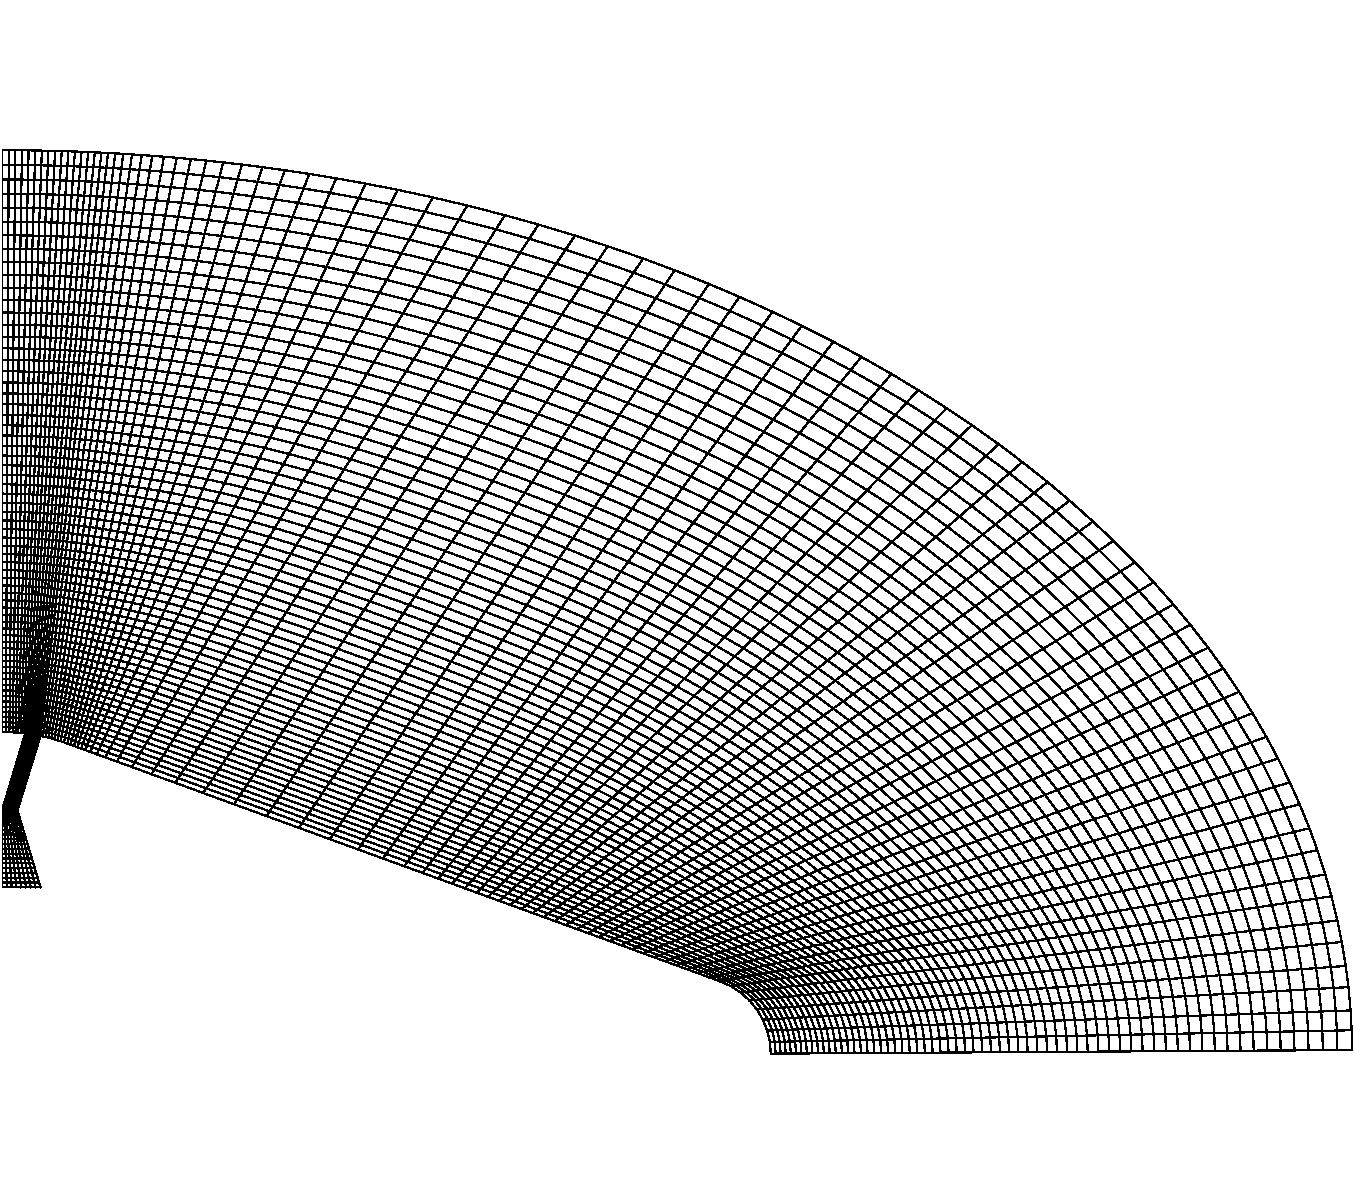
\includegraphics[width=0.5\textwidth]{srp_grid}
  \caption{SRP Configuration Grid}
  \label{fig:srp_grid}
\end{figure}
%------------------------------------------------------------------------------%
The nozzle parameters has a number of degrees of freedom with regard to user
input.  Combustion products can be specified separately from the freestream
flow, and will be mixed in as the solution progresses in time. Additionally, the
total pressure and temperature in the nozzle plenum can be specified.  Through
testing, this particular configuration has been determined to be steady and is
therefore a good candidate for testing with the adjoint.  In terms of
optimization, this case can be optimized for maximum drag, using a number of
design parameters.  The simplist design parameter is total pressure and/or
temperature in the nozzle plenum.  This results in a significant simplification
of the objective function to be minimized, because there is no mesh dependence
on the design variables; thus, eq.~(\ref{obj_function}) can be simplified to
%------------------------------------------------------------------------------%
\begin{equation}
  \frac{\partial L}{\partial \md}=
  \frac{\partial f}{\partial \md}
  +\frac{\partial \mr}{\partial \md}^T\mathbf{\Lambda}
  \label{simp_obj_func}
\end{equation}
%------------------------------------------------------------------------------%
Now the cost function and residual dependence upon the plenum initial conditions
must be derived.  For the drag cost function, this is achieved by looping over
all of the surface faces and linearizing the drag cost function w.r.t. the
pressure/temperature (CHECK THIS!).  For the residual, the 

\section{Specific Heat Derivatives}
\subsection{Linear Interpolation}

\textbf{NOTE: THIS IS NOT USED (we're quadratically interpolating)}
\vspace{4mm}

In order to check Specific heat ($C_p$) derivatives from the curve fits, $C_p$
and species enthalpy ($h_{ij}$) must have continuous derivatives.  This is not
inherently the case from the Gordon-McBride curve fits employed; therefore
blending is employed to ensure that both $C_p$ and $h_{ij}$ are $C_1$ and $C_0$
continuous.  The blending is implemented as
%------------------------------------------------------------------------------%
\begin{align}
  C_p &= f_n C_{p_n} + f_m C_{p_m} \\
  h_{ij} &= \int C_p dT = \int (f_n C_{p_n} + f_m C_{p_m}) dT
  \label{blending}
\end{align}
%------------------------------------------------------------------------------%
The curve fits defined by Gordon-McBride are a 7th-degree polynomial of the form
%------------------------------------------------------------------------------%
\begin{equation}
  C_p = \sum_{i=1}^{7} C_i T^{i-3}
  \label{cp_form}
\end{equation}
%------------------------------------------------------------------------------%
And the blending parameters, $f_n$ and $f_m$ are
%------------------------------------------------------------------------------%
\begin{gather}
  f_n = 
  \begin{cases}
    \frac{1}{2 dT_h} (T_u - T)  &(T_u - dT_h) < T \leq T_u \\
    \frac{1}{2 dT_l} (T - T_l)  &T_l < T \leq (T_l + dT_h)
  \end{cases} \\
  dT_h = \frac{T_u}{100} \quad dT_l = \frac{T_l}{100} \\
  f_m = 1 - f_n
  \label{blending_fxns}
\end{gather}
%------------------------------------------------------------------------------%
Where $T_u$ and $T_l$ are the upper and lower valid temperature bounds on a
range. Thus, substituting into eqn.~(\ref{blending}) yields
%------------------------------------------------------------------------------%
\begin{equation}
  h_{ij} = \int \left(f_n \sum_{i=1}^{7} C_{n_i} T^{i-3} + (1 - f_n) \sum_{i=1}^{7} C_{m_i} T^{i-3}\right) dT
  \label{semi-final}
\end{equation}
%------------------------------------------------------------------------------%
If $(T_u - dT_h) < T \leq T_u$, integrating eqn.~(\ref{semi-final}) yields
%------------------------------------------------------------------------------%
\begin{equation}
  h_{ij} = 50 h_n - \frac{50}{T_u}\left(C_{n_1}\ln(T) + \sum_{i=2}^{7} \frac{C_{n_i} T^{i-1}}{i-1} \right)
  -49 h_m + \frac{50}{T_u}\left(C_{m_1}\ln(T) + \sum_{i=2}^{7} \frac{C_{m_i} T^{i-1}}{i-1} \right) + C
  \label{up_low_range}
\end{equation}
%------------------------------------------------------------------------------%
Where
%------------------------------------------------------------------------------%
\begin{equation}
  h_n = \int C_{p_n} dT, \quad h_m = \int C_{p_m} dT
\end{equation}
%------------------------------------------------------------------------------%
If $T_l < T \leq (T_l + dT_h)$, integrating eqn.~(\ref{semi-final}) yields
%------------------------------------------------------------------------------%
\begin{equation}
  h_{ij} = -50 h_n + \frac{50}{T_l}\left(C_{n_1}\ln(T) + \sum_{i=2}^{7} \frac{C_{n_i} T^{i-1}}{i-1} \right)
  +49 h_m - \frac{50}{T_l}\left(C_{m_1}\ln(T) + \sum_{i=2}^{7} \frac{C_{m_i} T^{i-1}}{i-1} \right) + C
  \label{low_up_range}
\end{equation}
%------------------------------------------------------------------------------%
It quickly becomes apparent that eqn.s~(\ref{up_low_range}) and
(\ref{low_up_range}) can be combined into
%------------------------------------------------------------------------------%
\begin{equation}
  h_{ij} = \lambda\left[50 h_n - \frac{2}{dT_s}\left(C_{n_1}\ln(T) + \sum_{i=2}^{7} \frac{C_{n_i} T^{i-1}}{i-1} \right)
  -49 h_m + \frac{2}{dT_s}\left(C_{m_1}\ln(T) + \sum_{i=2}^{7} \frac{C_{m_i} T^{i-1}}{i-1} \right)\right] + C
  \label{final_w_const}
\end{equation}
%------------------------------------------------------------------------------%
with
%------------------------------------------------------------------------------%
\begin{equation}
  \lambda,\ dT_s = 
  \begin{cases}
    1,\ dT_u  &(T_u - dT_h) < T \leq T_u \\
    -1,\ dT_l &T_l < T \leq (T_l + dT_h)
  \end{cases} \\
\end{equation}
%------------------------------------------------------------------------------%
To detemine the constant of integration, $C$, we use the condition
%------------------------------------------------------------------------------%
\begin{equation}
  h_{ij}(T_{co}) = \frac{1}{2}(h_n(T_{co}) + h_m(T_{co})), \quad T_{co} = T_u = T_l
  \label{const_of_int}
\end{equation}
%------------------------------------------------------------------------------%
which specifies that the enthalpy at the intersection of temperature ranges
should the average of the enthalpy in the respective ranges.  Evaluating
eqn.~(\ref{final_w_const}) with condition provided my eqn.~(\ref{const_of_int})
yields
%------------------------------------------------------------------------------%
\begin{equation}
\begin{split}
  C &= (\frac{1}{2}-50\lambda)h_n\mid_{T=T_{co}}) + (\frac{1}{2}+49\lambda)h_m\mid_{T=T_{co}}) \\
  &+\frac{2\lambda}{dT_s}(C_{n_1}\ln(T_{co}) + \sum_{i=2}^{7} \frac{C_{n_i} T_{co}^{i-1}}{i-1}) \\
  &-\frac{2\lambda}{dT_s}(C_{m_1}\ln(T_{co}) + \sum_{i=2}^{7} \frac{C_{m_i} T_{co}^{i-1}}{i-1})
  \label{eval_const_int}
\end{split}
\end{equation}
%------------------------------------------------------------------------------%
Inserting into eq.~(\ref{eval_const_int}), the final form of the blended
enthalpy function is
%------------------------------------------------------------------------------%
\begin{equation}
  \begin{split}
    h_{ij} &= \lambda\left[50 h_n - \frac{2}{dT_s}\left(C_{n_1}\ln(T) + \sum_{i=2}^{7} \frac{C_{n_i} T^{i-1}}{i-1} \right)
    -49 h_m + \frac{2}{dT_s}\left(C_{m_1}\ln(T) + \sum_{i=2}^{7} \frac{C_{m_i} T^{i-1}}{i-1} \right)\right] \\
    &+ (\frac{1}{2}-50\lambda)h_n\mid_{T=T_{co}}) + (\frac{1}{2}+49\lambda)h_m\mid_{T=T_{co}}) \\
    &+\frac{2\lambda}{dT_s}\left(C_{n_1}\ln(T_{co}) + \sum_{i=2}^{7} \frac{C_{n_i} T_{co}^{i-1}}{i-1}\right) \\
    &-\frac{2\lambda}{dT_s}\left(C_{m_1}\ln(T_{co}) + \sum_{i=2}^{7} \frac{C_{m_i} T_{co}^{i-1}}{i-1}\right)
    \label{final}
  \end{split}
\end{equation}
%------------------------------------------------------------------------------%
\subsection{Quadratic Interpolation Between Thermodynamic Curve Fits}

We seek to blend the two thermodynamic curve fits in such a way that we maintain $c_0$ continuity in both specific heat ($C_p$) and enthalpy ($h$).  To accomplish this, a quadratic function must be used, of the form
%------------------------------------------------------------------------------%
\begin{equation}
  a T^2 + b T + c = C_p
  \label{generic_form}
\end{equation}
%------------------------------------------------------------------------------%
The coefficients $a$, $b$, and $c$ are determined by solving the system that results from the boundary value problem
%------------------------------------------------------------------------------%
\begin{equation}
  \begin{cases}
    a {T_1}^{2} + b T_1 +c = C_{p_1} \\
    a {T_2}^{2} + b T_2 +c = C_{p_2} \\
    a \frac{\left( {T_2}^{3} - {T_1}^{3}\right) }{3} + b\frac{ \left( {T_2}^{2} - {T_1}^{2}\right) }{2} + c \left( T_2 - T_1\right) = h_2-h_1
  \end{cases}
\end{equation}
%------------------------------------------------------------------------------%
Where the $x_1$ and $x_2$ subscripts describe the left and right states, respectively.  Solving the linear system, the coefficients are
%------------------------------------------------------------------------------%
\begin{myequation}
  \begin{cases}
    a=\frac{3\left( C_{p_2}+ C_{p_1}\right) }{(T_2-T_1)^{2}} - \frac{6 \left(h_2 - h_1\right)}{(T_2-T_1)^{3}}\\ \\
    b=-\frac{2\left[(C_{p_2} + 2C_{p_1})T_2 + (2C_{p_2} + C_{p_1})T_1\right]}{(T_2-T_1)^{2}} + \frac{6(T_2+T_1)(h_2 - h_1)}{(T_2 - T_1)^3}\\ \\
    c=\frac{C_{p_1} T_2 (T_2 + 2T_1) + C_{p_2} T_1 (T_1 + 2 T_2)}{(T_2-T_1)^2} - \frac{6 T_1 T_2 (h_2 - h_1)}{(T_2 - T_1)^3}
  \end{cases}
\end{myequation}
%------------------------------------------------------------------------------%
This can be simplified to
%------------------------------------------------------------------------------%
\begin{gather}
  \begin{cases}
    a=3B - A \\ \\
    b=\frac{-2(C_{p_1} T_2 + C_{p_2}T_2)}{(T_2 - T_1)^2} +(T_2+T_1) (A - 2B) \\ \\
    c=\frac{C_{p_1} {T_2}^2 + C_{p_2} {T_1}^2}{(T_2-T_1)^2} + T_1 T_2 (2B - A)
  \end{cases} \\
  A = \frac{6(h_2 - h_1)}{(T_2 - T_1)^3} \\
  B = \frac{C_{p_2} + C_{p_1}}{(T_2 - T_1)^2}
\end{gather}
%------------------------------------------------------------------------------%
\section{Block Jacobi Adjoint Decoupling}
%------------------------------------------------------------------------------%
% Decoupled adjoint derivation content
%------------------------------------------------------------------------------%

The primal flow equations are solved using the decoupled scheme based on the
work by Candler, et. al.  In doing this the conserved variables are split from
%------------------------------------------------------------------------------%
\begin{equation}
	\vU =
  \begin{pmatrix}
 		\rho_1    \\
		\vdots    \\
		\rho_{ns} \\
		\rho u    \\
		\rho v    \\
		\rho w    \\
		\rho E    \\
	\end{pmatrix}
  \label{all-vars}
 \end{equation}
%------------------------------------------------------------------------------%
 into
%------------------------------------------------------------------------------%
\begin{equation}
	\begin{matrix}
		\mathbf{U}'=\begin{pmatrix}
			\rho \\
			\rho u \\
			\rho v \\
			\rho w \\
			\rho E
		\end{pmatrix},\quad &
		\mathbf{\hat{U}}=\begin{pmatrix}
			\rho_1 \\
			\vdots \\
			\rho_{ns}
		\end{pmatrix}
	\end{matrix}
  \label{dc-vars}
\end{equation}
%------------------------------------------------------------------------------%
By doing this, the flow equations can be solved implicitly using an approximate,
first-order jacobian to drive the flow solution to a converged steady-state.  In
practice, this is done by essentially formulating
%------------------------------------------------------------------------------%
\begin{equation}
  \frac{V}{\Delta t}\mi + 
  \begin{pmatrix}
    \rdiff{\rho}{\rho} & \rdiff{\rho}{\rho \vu} & \rdiff{\rho}{\rho E} \\ \\
    \rdiff{\rho \vu}{\rho} & \rdiff{\rho \vu}{\rho \vu} & \rdiff{\rho \vu}{\rho E} \\ \\
    \rdiff{\rho E}{\rho} & \rdiff{\rho E}{\rho \vu} & \rdiff{\rho E}{\rho E}
  \end{pmatrix}
  \begin{pmatrix}
    \Delta \rho \\ \\
    \Delta \rho \vu \\ \\
    \Delta \rho E
  \end{pmatrix}
  =
  \begin{pmatrix}
    \res{\rho} \\ \\
    \res{\rho \vu} \\ \\
    \res{\rho E}
  \end{pmatrix}
  \label{approx-jac}
\end{equation}
%------------------------------------------------------------------------------%
to solve for the mixture flow variables, and formulating
%------------------------------------------------------------------------------%
\begin{equation}
  \frac{V}{\Delta t}\mi + 
  \begin{pmatrix}
    \rdiff{\rho_1}{c_1} & \cdots & \rdiff{\rho_{1}}{c_{ns}} \\ \\
    \vdots & \ddots & \vdots \\ \\
    \rdiff{\rho_{ns}}{c_1} & \cdots & \rdiff{\rho_{ns}}{c_{ns}}
  \end{pmatrix}
  \begin{pmatrix}
    \Delta c_1 \\ \\
    \vdots \\ \\
    \Delta c_{ns}
  \end{pmatrix}
  =
  \begin{pmatrix}
    \res{\rho_1} \\ \\
    \vdots \\ \\
    \res{\rho_{ns}}
  \end{pmatrix}
  \label{approx-jac-dc}
\end{equation}
%------------------------------------------------------------------------------%
Note that the correction terms required to maintain $\lsum{s=1}{ns}{c_s} = 1$
and $\lsum{s=1}{ns}{\delta c_s} = 0$ are omitted in \eref{approx-jac-dc} only
for brevity in this explanation.  Examining \erefs{approx-jac}{approx-jac-dc}
shows that there are clearly some physical dependencies being omitted, namely
$\rdiff{\rho_s}{\rho}$, $\rdiff{\rho}{c_s}$, $\rdiff{\rho \vu}{c_s}$, and 
$\rdiff{\rho E}{c_s}$.  It has been demonstrated that omitting this dependencies
does not hinder convergence the primal solver; however, the adjoint requires an
exact linearization of the converged steady-state solution.

The discrete adjoint formulation is given as
%------------------------------------------------------------------------------%
\begin{equation}
  \bigg[\rdiff{}{\mq}\bigg]^T\mathbf{\Lambda}= -\pd{f}{\mq}
  \label{adjoint}
\end{equation}
%------------------------------------------------------------------------------%
where $\mq$ is a vector of conserved variables, and $f$ is the cost function (i.e.
lift, drag, etc.). There is now an apparent need to reconcile the two sets of
conserved variables in \eref{dc-vars} with $\mq$.  The most intuitive and
staightforward way to do this is to forgo solving for the species mass $\rho_s$
in lieu of the species mass fraction $c_s$.  Thus, $\mq$ can be expressed as
%------------------------------------------------------------------------------%
\begin{equation}
  \mq =
  \begin{pmatrix}
  	\rho \\
  	\rho u \\
  	\rho v \\
  	\rho w \\
  	\rho E \\
    c_1 \\
    \vdots \\
    c_{ns}
  \end{pmatrix}
  \label{q-vec}
\end{equation}
%------------------------------------------------------------------------------%
This allows the linearizations derived in \erefs{approx-jac}{approx-jac-dc} to
be used in the adjoint formulation, by augmenting them with the previously
omitted linearizations.  Replacing $\rdiff{}{\mq}$ with the fully system, the
adjoint system becomes
%------------------------------------------------------------------------------%
\begin{equation}
  \begin{pmatrix}
    \rtdiff{\rho}{\rho} & \rtdiff{\rho}{\rho \vu} & 
    \rtdiff{\rho}{\rho E} & \rtdiff{\rho}{c_s} \\ \\
    \rtdiff{\rho \vu}{\rho} & \rtdiff{\rho \vu}{\rho \vu} & 
    \rtdiff{\rho \vu}{\rho E} & \rtdiff{\rho \vu}{c_s} \\ \\
    \rtdiff{\rho E}{\rho} & \rtdiff{\rho E}{\rho \vu} & 
    \rtdiff{\rho E}{\rho E} & \rtdiff{\rho E}{c_s} \\ \\
    \rtdiff{\rho_s}{\rho} & \rtdiff{\rho_s}{\rho \vu} & 
    \rtdiff{\rho_s}{\rho E} & \rtdiff{\rho_s}{c_s}
  \end{pmatrix}
  \begin{pmatrix}
    \adjlam{\rho} \\ \\
    \adjlam{\rho \vu} \\ \\
    \adjlam{\rho E} \\ \\
    \adjlam{c_s}
  \end{pmatrix}
  = -
  \begin{pmatrix}
    \pd{f}{\rho} \\ \\
    \pd{f}{\rho \vu} \\ \\
    \pd{f}{\rho E} \\ \\
    \pd{f}{c_s}
  \end{pmatrix}
  \label{full-adjoint}
\end{equation}
%------------------------------------------------------------------------------%
Thus the jacobian in \eref{full-adjoint} is the completed one of
\erefs{approx-jac}{approx-jac-dc}.  While this is useful, the point of
decoupling the species equations from the mixture equations was to speed up the
linear solver and save memory.  Solving \eref{full-adjoint} undermines both of
these goals, so an alternative solution strategy must be formulated.  If a block
jacobi scheme is employed, the system can be decoupled once again as
%------------------------------------------------------------------------------%
\begin{equation}
  \begin{pmatrix}
    \rtdiff{\rho}{\rho} & \rtdiff{\rho}{\rho \vu} & \rtdiff{\rho}{\rho E} \\ \\
    \rtdiff{\rho \vu}{\rho} & \rtdiff{\rho \vu}{\rho \vu} & \rtdiff{\rho \vu}{\rho E} \\ \\
    \rtdiff{\rho E}{\rho} & \rtdiff{\rho E}{\rho \vu} & \rtdiff{\rho E}{\rho E}
  \end{pmatrix}
  \begin{pmatrix}
    \adjlam{\rho} \\ \\
    \adjlam{\rho \vu} \\ \\
    \adjlam{\rho E}
  \end{pmatrix}
  = -
  \begin{pmatrix}
    \pd{f}{\rho} \\ \\
    \pd{f}{\rho \vu} \\ \\
    \pd{f}{\rho E}
  \end{pmatrix}
  -
  \begin{pmatrix}
    \rtdiff{\rho}{c_s} \\ \\
    \rtdiff{\rho \vu}{c_s} \\ \\
    \rtdiff{\rho E}{c_s}
  \end{pmatrix}
  \adjlam{c_s}
  \label{dc-adjoint-1}
\end{equation}
%------------------------------------------------------------------------------%
\begin{equation}
  \rtdiff{\rho_s}{c_s}
  \adjlam{c_s}
  = -\pd{f}{c_s}
  - \rtdiff{\rho_s}{\rho} \adjlam{\rho}
  - \rtdiff{\rho_s}{\rho \vu} \adjlam{\rho \vu}
  - \rtdiff{\rho_s}{\rho E} \adjlam{\rho E}
  \label{dc-adjoint-2}
\end{equation}
%------------------------------------------------------------------------------%
If a time-like derivative is added to the adjoint, the solution of the costate
variables, $\Lambda$, can be time marched similar to the primal flow solver
%------------------------------------------------------------------------------%
\begin{equation}
  \left[ \frac{V}{\Delta t} \mi + \rtdiff{}{\mq} \right] \Delta
  \adjlam{}
  = -\pd{f}{\mq} - \rtdiff{}{\mq} \adjlam{}
  \label{adj-dc-time-general}
\end{equation}
%------------------------------------------------------------------------------%
Thus, the first system in \eref{dc-adjoint-1} becomes
%------------------------------------------------------------------------------%
\begin{equation}
  \begin{split}
    \left[
      \frac{V}{\Delta t} \mi +
      \begin{pmatrix}
        \rtdiff{\rho}{\rho} & \rtdiff{\rho}{\rho \vu} & \rtdiff{\rho}{\rho E} \\ \\
        \rtdiff{\rho \vu}{\rho} & \rtdiff{\rho \vu}{\rho \vu} & \rtdiff{\rho \vu}{\rho E} \\ \\
        \rtdiff{\rho E}{\rho} & \rtdiff{\rho E}{\rho \vu} & \rtdiff{\rho E}{\rho E}
      \end{pmatrix}
    \right]
    \begin{pmatrix}
      \Delta \adjlam{\rho} \\ \\
      \Delta \adjlam{\rho \vu} \\ \\
      \Delta \adjlam{\rho E}
    \end{pmatrix}
    &= \\ -
    \begin{pmatrix}
      \pd{f}{\rho} \\ \\
      \pd{f}{\rho \vu} \\ \\
      \pd{f}{\rho E}
    \end{pmatrix}
    -
    \begin{pmatrix}
      \rtdiff{\rho}{\rho} & \rtdiff{\rho}{\rho \vu} & \rtdiff{\rho}{\rho E} \\ \\
      \rtdiff{\rho \vu}{\rho} & \rtdiff{\rho \vu}{\rho \vu} & \rtdiff{\rho \vu}{\rho E} \\ \\
      \rtdiff{\rho E}{\rho} & \rtdiff{\rho E}{\rho \vu} & \rtdiff{\rho E}{\rho E}
    \end{pmatrix}
    &
    \begin{pmatrix}
      \adjlam{\rho} \\ \\
      \adjlam{\rho \vu} \\ \\
      \adjlam{\rho E}
    \end{pmatrix}
    -
    \begin{pmatrix}
      \rtdiff{\rho}{c_s} \\ \\
      \rtdiff{\rho \vu}{c_s} \\ \\
      \rtdiff{\rho E}{c_s}
    \end{pmatrix}
    \adjlam{c_s}
  \end{split}
  \label{adj-dc-time1}
\end{equation}
%------------------------------------------------------------------------------%
and the second system in \eref{dc-adjoint-2} becomes
%------------------------------------------------------------------------------%
\begin{equation}
  \left( \frac{V}{\Delta t} \mi + \rtdiff{\rho_s}{c_s} \right) \Delta
  \adjlam{c_s}
  = \\ -\pd{f}{c_s}
  - \rtdiff{\rho_s}{c_s} \adjlam{c_s}
  - \rtdiff{\rho_s}{\rho} \adjlam{\rho}
  - \rtdiff{\rho_s}{\rho \vu} \adjlam{\rho \vu}
  - \rtdiff{\rho_s}{\rho E} \adjlam{\rho E}
  \label{adj-dc-time2}
\end{equation}
%------------------------------------------------------------------------------%
This is advantageous, because the jacobians on the left hand side (LHS) can be
the first-order approximate jacobians that were used to solve the primal flow
equations; hence, all of the benefits of the diagonal block matricies that are
exploited to reduce the linear solver cost and overall memory now apply to the
adjoint.

\end{document}  
